\documentclass{standalone}

\usepackage{tikz}

\usetikzlibrary{positioning}
\usetikzlibrary{decorations}
\usetikzlibrary{decorations.markings}
\usetikzlibrary{decorations.text}

\begin{document}
  %noformat{
  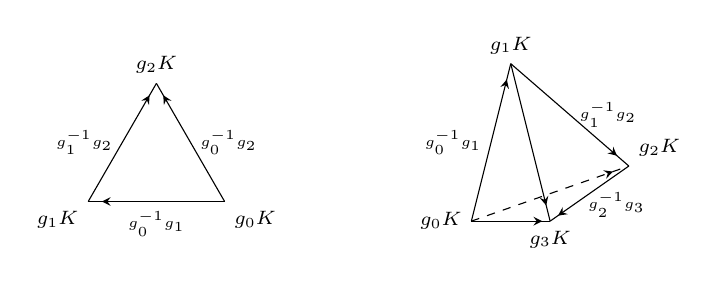
\begin{tikzpicture}
    \tikzstyle{e} = [postaction=decorate, decoration={markings, mark=at position 0.9 with {\arrow{stealth}}}]

    \tikzset{font=\scriptsize}

    \begin{scope}[shift={(0,0.75)}]
      \coordinate[label=330:{$g_0K$}] (v0) at (330:1.0);
      \coordinate[label=210:{$g_1K$}] (v1) at (210:1.0);
      \coordinate[label= 90:{$g_2K$}] (v2) at ( 90:1.0);

      \draw[e] (v0) to node[midway, below] (t01) {\tiny $g_0^{-1} g_1$} (v1);
      \draw[e] (v0) to node[midway, right] (t02) {\tiny $g_0^{-1} g_2$} (v2);
      \draw[e] (v1) to node[midway, left ] (t12) {\tiny $g_1^{-1} g_2$} (v2);
    \end{scope}

    \begin{scope}[shift={(4,0)}]
      \coordinate[label=180:{$g_0K$}] (v0) at (0.0,0.0);
      \coordinate[label= 90:{$g_1K$}] (v1) at (0.5,2.0);
      \coordinate[label= 30:{$g_2K$}] (v2) at (2.0,0.7);
      \coordinate[label=270:{$g_3K$}] (v3) at (1.0,0.0);

      \draw[e] (v0) to node[midway, left] (t01) {\tiny $g_0^{-1} g_1$} (v1);
      \draw[dashed, e] (v0) to (v2);
      \draw[e] (v0) to (v3);
      \draw[e] (v1) to node[midway, right] (t12) {\tiny $g_1^{-1} g_2$} (v2);
      \draw[e] (v1) to (v3);
      \draw[e] (v2) to node[midway, below right=-0.2] (t23) {\tiny $g_2^{-1} g_3$} (v3);
    \end{scope}
  \end{tikzpicture}
  %}noformat
\end{document}
